\documentclass{article}

% Use [final] for the submitted course report
\usepackage[final]{neurips_2024}

\usepackage[utf8]{inputenc}
\usepackage[T1]{fontenc}
\usepackage[colorlinks=true,linkcolor=blue!60!black,citecolor=blue!60!black,urlcolor=blue!60!black]{hyperref}
\usepackage{url}
\usepackage{booktabs}
\usepackage{amsfonts}
\usepackage{amsmath}
\usepackage{amssymb}
\usepackage{nicefrac}
\usepackage{microtype}
\usepackage{xcolor}
\usepackage{graphicx}
\usepackage{subcaption}
\usepackage{multirow}
\usepackage{enumitem}
\usepackage{tikz}
\usetikzlibrary{arrows.meta,positioning,calc}

% Helper command for TODOs / Plan C placeholders (remove before final submission)
\newcommand{\todo}[1]{\textcolor{red!75!black}{\textbf{[TODO: #1]}}}
\newcommand{\planc}[1]{\textcolor{orange!80!black}{\textbf{[Plan C Slot: #1]}}}

\title{What Should a Slow Planner Tell a Fast Dexterous Hand?\\
Content, Rate, and Validity Windows in Low-Dimensional Intent Interfaces}

\author{%
  Team 34 (Author Names Here) \\
  School of Computing, National University of Singapore \\
  \texttt{\{email1, email2\}@u.nus.edu} \\
  \vspace{0.3em}
  \textbf{Code:} \url{https://github.com/ziyouledi/CS5478_project}
}

\begin{document}

\maketitle

\begin{abstract}
Vision-language models (VLMs) plan at 0.2--2~Hz, whereas dexterous robotic hands require 60~Hz closed-loop motor control.
Bridging this gap requires a low-dimensional \emph{intent interface} between a slow planner and a fast low-level controller, yet it remains unclear what representation should cross this channel under realistic rate, latency, and precision limits.
We systematically benchmark three abstraction levels---action synergies, object waypoints, and goal-level commands---across three Shadow Hand tasks in Isaac Lab: 3D cube reorientation, $z$-axis rotation, and a simplified Rubik's-like cube combining whole-cube reorientation with $\pm 90^\circ$ top-layer twists.
While 8-D action synergies match goal commands at 60~Hz (87\% expert recovery), reducing the update rate to $\le 10$~Hz or adding $\ge 0.1$~s latency triggers a sharp reversal: inter-update staleness collapses action and waypoint interfaces, leaving goal commands (at $\ge 8$~bits/component) as the sole representation that degrades predictably along an analytical waiting-time law, $P(d) \approx 600/(T_0 + d)$.
Guided by this principle, we train a unified 60~Hz multi-skill controller (\texttt{Unified v4}) that holds the cube through 4~s planner pauses with zero drops, and pair it with an open-weight 8B VLM (\texttt{Qwen3-VL-8B-Instruct}) adapted via lightweight Map-then-Reason LoRA (0.51\% trainable parameters, frozen ViT).
Across 128 real-time 60~Hz closed-loop episodes in Isaac Lab, the resulting system achieves \textbf{100.0\%} task completion with zero drops, showing that a goal-level interface turns a slow, open-weight VLM into a reliable dexterous-hand planner.
\end{abstract}


\section{Introduction}
\label{sec:intro}

General-purpose large language and vision-language models (LLMs/VLMs) are rapidly emerging as high-level robot planners, capable of interpreting visual scenes and reasoning over multi-step manipulation tasks \citep{mirchandani2023llms,tang2026training}.
Yet these models face a fundamental systems constraint: autoregressive decoding takes hundreds of milliseconds to several seconds per decision (0.2--2~Hz), whereas multi-fingered dexterous hands performing contact-rich in-hand manipulation require closed-loop feedback at 60~Hz or higher \citep{andrychowicz2020learning,akkaya2019solving}.
For robot arms with parallel grippers, off-the-shelf inverse kinematics (IK) and pose controllers bridge this gap cleanly, allowing a slow model to output sparse end-effector poses \citep{tang2026training}.
For a 20-DOF anthropomorphic hand, no standard low-frequency execution layer exists.
Instead, a slow high-level planner must communicate with a fast pre-trained low-level controller across a rate-limited \emph{intent interface}.

This raises a central design question: \textbf{what representation should cross the intent channel between a slow planner and a fast dexterous hand, and how does channel degradation—low refresh rate, transmission latency, and quantization—determine which representations remain viable?}
Prior studies typically commit to a single interface level (e.g., hand synergies, wrist keypoints, or discrete skills) and evaluate it at a fixed control frequency.
Consequently, the interaction between \emph{intent abstraction level} and \emph{channel rate/latency} remains poorly understood.

To answer this question, we conduct a two-part study on the 20-DOF Shadow Hand in Isaac Lab \citep{mittal2023orbit} spanning three tasks of increasing complexity (3D reorientation, $z$-axis rotation, and a simplified Rubik's-like cube).
First, we isolate the information carried by the intent channel using a goal-hidden asymmetric-critic student protocol \citep{pinto2018asymmetric}, comparing \emph{action-level}, \emph{object-subgoal}, and \emph{goal-level} interfaces across controlled refresh-rate, latency, and quantization sweeps.
Second, guided by these findings, we instantiate an end-to-end VLM manipulation system: we pair a frozen 60~Hz multi-skill controller with an open-weight 8B VLM adapted via Map-then-Reason LoRA SFT and closed-loop GRPO \citep{shao2024deepseekmath}, evaluating perception generalization, planning efficiency, and real-time 60~Hz physical execution.

Our main contributions are fourfold:
\begin{enumerate}[leftmargin=1.5em,itemsep=1.5pt,topsep=2pt]
  \item \textbf{Full-rate bandwidth and action diagnostics (Task 1).} On 3D cube reorientation, RL policies exhibit a flat action spectrum (8~PCs for 81\% variance vs.\ 2 in human grasping \citep{santello1998postural}), and \texttt{hand-8} matches goal-level commands at 60~Hz (87\% vs.\ 78\% recovery).
  \item \textbf{Rate reversal and staleness laws (Tasks 1--2).} On both reorientation tasks, $\le 10$~Hz refresh or $\ge 0.1$~s latency collapses action and waypoint intents while goal commands follow an analytical waiting-time law $P(d)\approx 600/(T_0+d)$ ($\sim 32$~bits/goal); a slow-expert control confirms the hand itself must stay fast, and $z$-axis rotation exposes a \emph{stale-goal trap} below blind spinning.
  \item \textbf{Multi-skill controller and Task 3 boundary conditions.} We train a unified 60~Hz hinged-cube policy (\texttt{Unified v4}, $2.4\times$ faster than two-expert handoff) where multi-skill switching reproduces the 10~Hz reversal, whereas on isolated 1-DOF face turns outcomes are bimodal and seed-driven rather than rate-driven at 10~Hz because held \texttt{hand-8} retains goal-direction information.
  \item \textbf{End-to-end VLM control.} Pairing frozen \texttt{Unified v4} (100\% BFS execution, 4~s pause stability) with \texttt{Qwen3-VL-8B-Instruct} via lightweight Map-then-Reason LoRA SFT (0.51\% parameters, frozen ViT) achieves 100.0\% (128/128) real-time 60~Hz closed-loop manipulation in Isaac Lab with zero drops.
\end{enumerate}

\section{Related Work}
\label{sec:related}

\subsection{In-Hand Manipulation and Hand Synergies}
GPU-accelerated RL enables anthropomorphic hands to perform in-hand cube reorientation \citep{andrychowicz2020learning,mittal2023orbit} and Rubik's-cube solving \citep{akkaya2019solving} via PPO \citep{schulman2017proximal,makoviichuk2021rlgames} and asymmetric actor-critic training \citep{pinto2018asymmetric}.
In parallel, hand-synergy studies showed that two principal components capture $>80\%$ of static human grasping variance \citep{santello1998postural}, inspiring eigengrasp planning \citep{ciocarlie2009hand}, multi-task motor priors \citep{caggiano2023myodex,yuan2025crossdex}, wrist--finger decoupling \citep{liu2016analysis,jarquebou2019kinematic}, and synergy complexity indices \citep{west2025synergy}.
However, prior synergy work examines \emph{spatial} dimensionality only at full control rates, leaving open how action codes behave under slow updates.

\subsection{Hierarchical Interfaces, Skill Composition, and Frequency Decoupling}
To bridge slow high-level planning and fast motor control, visuomotor methods such as action chunking \citep{zhao2023learning} and diffusion policies \citep{chi2023diffusion} execute multi-step action sequences open-loop to amortize inference, while dual-system VLAs and hierarchical hand policies connect VLMs to fast controllers via latent action codes or 3D keypoints \citep{chen2025fastinslow,jiang2026xlvla,debakker2025scaffolding}.
Yet open-loop chunks are fragile under contact-rich, high-switching in-hand dynamics, and existing systems commit to a single interface abstraction without head-to-head sweeps across refresh rate, latency, and quantization.
A related design axis is how multiple dexterous skills are organized at the low level: chaining or composing separate specialist policies via transition feasibility or residual adapters \citep{chen2023sequential,huang2026dexcompose} versus distilling a single unified low-level controller \citep{yin2025dexteritygen}.
Our study benchmarks both axes on the same hand---sweeping interface abstraction under channel degradation (Part~I) and directly comparing two-expert handoff against a unified 60~Hz controller (Part~II).

\subsection{VLMs as High-Level Robot Planners}
LLMs and VLMs increasingly serve as high-level robot planners through affordance grounding \citep{ichter2022saycan}, pattern extrapolation \citep{mirchandani2023llms}, vision-language-action co-training \citep{brohan2023rt2}, and outcome-based RL via GRPO \citep{shao2024deepseekmath,tang2026training}.
On robot arms, sparse VLM commands succeed because off-the-shelf IK/pose controllers execute fast motions between queries \citep{tang2026training}; on dexterous hands, recent VLAs mainly target grasping \citep{zhong2026dexgraspvla}, whereas direct slow joint control by frontier models largely fails on in-hand manipulation \citep{galbot2026astra}.
Even with a capable low-level controller, open-weight VLMs exhibit fine-grained multi-view spatial deficits on BLINK \citep{fu2024blink}, MMStar \citep{chen2024mmstar}, and EmbSpatial \citep{du2024embspatial}.
Existing remedies rely on visual overlays \citep{yang2023setofmark,nasiriany2024pivot} or tool-augmented 3D spatial reasoning \citep{zhang2026think3d,li2026skill3d}, which introduce external dependencies or extra inference latency; our Part~II system instead pairs a frozen 60~Hz goal-conditioned controller with lightweight Map-then-Reason LoRA adaptation for single-pass, marker-free closed-loop control.

\section{Problem Formulation and Method}
\label{sec:method}

\subsection{Overview: Seven-Step Pipeline and Dual Role of the Expert}
\label{sec:method_overview}
Our methodology spans two tightly linked parts---\textbf{Part~I (Steps~1--5)}: a controlled benchmark of low-dimensional intent interfaces under channel degradation, and \textbf{Part~II (Steps~6--7)}: deploying the winning goal-level interface in an end-to-end VLM manipulation system:
\begin{enumerate}[leftmargin=1.5em,itemsep=1.5pt,topsep=2pt]
  \item \textbf{Step~1 (Reference expert training \& freezing):} Train a goal-visible PPO policy per task and freeze its final checkpoint to define the 100\% performance ceiling $P_E$.
  \item \textbf{Step~2 (Deterministic rollout \& PCA basis):} Roll out the frozen reference expert to collect 1.23M continuous transitions and fit orthogonal action-synergy PCA bases $W$.
  \item \textbf{Step~3 (Intent generation \& channel degradation):} At each step, compute a $k$-D intent $z_t$ (action, object-subgoal, or goal level) and pass it through controlled zero-order hold, delay, or quantization to obtain $\tilde{z}_t$.
  \item \textbf{Step~4 (Goal-hidden student training):} Strip goal observations from the actor and train a goal-hidden student via asymmetric-critic PPO using $\tilde{z}_t$ as its sole task cue, executing all interface and rate/delay sweeps here.
  \item \textbf{Step~5 (Deterministic evaluation):} Evaluate all 25 periodic checkpoints across 1,024 fixed-seed episodes to compute exact completions, recovery, staleness, and waiting-time fits.
  \item \textbf{Step~6 (Unified 60~Hz multi-skill controller):} Train a single goal-conditioned controller (\texttt{Unified v4}) for the two-skill hinged cube and verify its 96-state BFS execution ceiling and 4~s pause stability.
  \item \textbf{Step~7 (Upstream VLM adaptation \& online 60~Hz loop):} Adapt \texttt{Qwen3-VL-8B-Instruct} via Map-then-Reason LoRA SFT and closed-loop GRPO to drive frozen \texttt{Unified v4} from live 3-camera images.
\end{enumerate}

\paragraph{Clarifying the dual role of the expert.}
To avoid ambiguity, note that the frozen expert serves \emph{two distinct roles} across Parts~I and~II.
In \textbf{Part~I (Steps~1--5)}, it is a \textbf{Reference Expert}: it sets the $P_E$ baseline, supplies the offline PCA basis, and—\emph{only} for action-level intents—acts online as an action-intent oracle computing $a_t^E \to z_t$.
Crucially, student training in Step~4 is \emph{not} teacher--student action distillation; every student learns autonomously from environment rewards via asymmetric-critic PPO.
In \textbf{Part~II (Steps~6--7)}, once Part~I establishes that slow planners must emit goal-level commands, frozen \texttt{Unified v4} serves directly as the \textbf{60~Hz Goal-Conditioned Skill Controller} (analogous to an arm's IK controller) executed under the slow VLM planner.

\subsection{Tasks, Simulation Setup, and Evaluation Protocol}
\label{sec:method_tasks}
All experiments run in Isaac Lab v2.3.1 \citep{mittal2023orbit} on the 24-DOF Shadow Dexterous Hand (20 actuated joints: 2 wrist drives at action indices 0--1 and 18 finger drives at indices 2--19, with 4 coupled distal joints).
Physics runs at 120~Hz with decimation 2, yielding a 60~Hz discrete-time control loop and 10~s episodes (600 control steps) with continuous observations $s_t \in \mathbb{R}^{157}$ and continuous actions $a_t \in [-1,1]^{20}$.
Observations include joint positions/velocities, object pose/velocities, goal quaternion \texttt{obs[64:68]}, relative object--goal quaternion \texttt{obs[68:72]}, fingertip states, and previous action.
We evaluate three tasks of increasing complexity:
\begin{itemize}[leftmargin=1.5em,itemsep=1.5pt,topsep=2pt]
  \item \textbf{Task~1 ($\mathrm{SO}(3)$ Reorientation):} Standard \texttt{Isaac-Repose-Cube-Shadow-Direct-v0}. Reorient a 6~cm cube to random 3D target orientations within 0.1~rad; each success samples a new target without resetting the hand ($P_E=26.11$).
  \item \textbf{Task~2 ($z$-Axis Reorientation, M2):} \texttt{Isaac-Repose-Cube-Shadow-ZAxis-Direct-v0}, restricting targets to yaw rotations about the palm-normal $z$-axis ($P_E=31.14$).
  \item \textbf{Task~3 (Simplified Rubik's-Like Hinged Cube):} A custom two-part 6~cm cube (0.216~kg, friction 1.0) whose top third twists about the cube $z$-axis against a 0.05~N$\cdot$m detent torque cap every $90^\circ$. It combines whole-cube reorientation (\texttt{any}: arbitrary 3D target; \texttt{up}: top layer upright with random yaw) and $\pm 90^\circ$ top-layer twists (\texttt{turn}: hinge within 0.1~rad of target for 10 consecutive steps, 0.17~s).
\end{itemize}

\paragraph{Exact per-episode evaluation (Step~5).}
Because Isaac Lab's built-in \texttt{consecutive\_successes} metric is an across-reset exponential moving average that understates throughput ($\approx 15.5$ vs.\ $26.11$), all results use an independent deterministic evaluator over 1,024 fixed-seed episodes per checkpoint, reporting exact per-episode completions $P$, drop rate, and normalized recovery:
\begin{equation}
  \mathrm{Recovery}(c) = \frac{P(c) - P_{\mathrm{blind}}}{P_E - P_{\mathrm{blind}}},
  \label{eq:recovery}
\end{equation}
where $P_{\mathrm{blind}}$ is the goal-hidden student with no intent ($0.006$ on Task~1; $19.66$ on Task~2).
Policies train with RL-Games PPO \citep{schulman2017proximal,makoviichuk2021rlgames} for 5,000 iterations (2,048 envs, 163.84M transitions; 8,192 envs on H200 for unified experts), with 3--5 seeds per condition and two-sided Welch $t$- / Mann--Whitney $U$ tests.

\subsection{Goal-Hidden Student Training and Intent Taxonomy (Steps 1--4)}
\label{sec:method_student}
In a preliminary goal-visible stage (Stage~1; 21 runs on Task~1 and 30 on Task~2), appending intents to a goal-visible actor yielded no significant speed or AUC gain (one-way ANOVA N80 $p=0.82$, AUC $p=0.65$; Appendix~\ref{app:stage1}), because the actor already observes the goal directly.
To isolate the information carried by the intent channel, we adopt a \emph{goal-hidden asymmetric-critic} protocol (Figure~\ref{fig:protocol}): the 8 goal fields \texttt{obs[64:72]} are stripped from the student actor (leaving 149-D proprioceptive/object state plus the $k$-D intent $\tilde{z}_t$), while the central value critic \citep{pinto2018asymmetric} retains the full 157-D state during training for low-variance advantage estimation.
A goal-visible asymmetric-critic gate run matches the symmetric expert within 1.4\% ($25.76 = 0.986\,P_E$), confirming no architectural confound.

\begin{figure}[t]
  \centering
  % Compact TikZ diagram for Figure 1 (v2): Part I Student Training & Channel-Sweep Architecture (Steps 1--5)
% Explicitly decomposes: 157-D -> Frozen Expert -> 20-D action -> Fixed Offline PCA Projection -> k-D intent,
% explicit Concat(149-D physical state, z_tilde), and solid-line Asymmetric Critic for all training conditions.
\definecolor{navink}{HTML}{17213A}
\definecolor{mutedgray}{HTML}{62708D}
\definecolor{cardbg}{HTML}{F6F8FC}
\definecolor{cardborder}{HTML}{CBD5E1}
\definecolor{intentblue}{HTML}{2C67F2}
\definecolor{intentbluebg}{HTML}{EEF4FF}
\definecolor{chanorange}{HTML}{D9602F}
\definecolor{chanorangebg}{HTML}{FFF3ED}
\definecolor{criticgreen}{HTML}{1E9C77}
\definecolor{criticgreenbg}{HTML}{EDF9F5}
\definecolor{stripcrimson}{HTML}{C62828}

\resizebox{\linewidth}{!}{%
\begin{tikzpicture}[
    font=\sffamily\footnotesize,
    >=Stealth,
    box/.style={
      rectangle, rounded corners=3.5pt, draw=cardborder, fill=cardbg,
      line width=0.85pt, align=center, inner sep=3.5pt, text=navink
    },
    envbox/.style={
      box, draw=navink!70, fill=cardbg, line width=1.0pt,
      minimum width=2.45cm, minimum height=1.85cm
    },
    expertbox/.style={
      box, draw=navink!65, fill=cardbg, line width=0.95pt,
      minimum width=2.7cm, minimum height=0.82cm
    },
    pcabox/.style={
      box, draw=intentblue!85, fill=intentbluebg, line width=0.95pt,
      minimum width=2.9cm, minimum height=0.82cm
    },
    basisbox/.style={
      box, draw=mutedgray, fill=white, dashed, line width=0.8pt,
      minimum height=0.48cm, inner sep=3pt
    },
    chanbox/.style={
      box, draw=chanorange, fill=chanorangebg, line width=1.0pt,
      minimum width=3.6cm, minimum height=0.82cm
    },
    actorbox/.style={
      box, draw=intentblue, fill=intentbluebg, line width=1.05pt,
      minimum width=3.6cm, minimum height=0.95cm
    },
    criticbox/.style={
      box, draw=criticgreen, fill=criticgreenbg, line width=1.0pt,
      minimum width=3.6cm, minimum height=0.88cm
    },
    concatnode/.style={
      circle, draw=intentblue, fill=intentbluebg, line width=1.0pt,
      inner sep=1.2pt, minimum size=0.46cm, font=\sffamily\small\bfseries, text=intentblue
    },
    wire/.style={->, line width=0.9pt, draw=navink!80},
    criticwire/.style={->, line width=0.95pt, draw=criticgreen!90!black},
    dashwire/.style={->, dashed, line width=0.8pt, draw=mutedgray},
    stripwire/.style={-, dashed, line width=0.9pt, draw=stripcrimson}
  ]

  % Main nodes (vertically compacted to save page height)
  \node[envbox] (env) at (-0.35, 1.30) {
    \textbf{Isaac Lab Env}\\[1.5pt]
    {\scriptsize Shadow Hand}\\
    {\scriptsize 60~Hz ctrl (600 steps)}
  };

  % Top row: 157-D -> Frozen Expert -> 20-D action -> Online PCA Proj -> Intent Channel
  \node[expertbox] (expert) at (5.05, 3.15) {
    \textbf{Frozen Expert $\pi_E$}\\[0.5pt]
    {\scriptsize Step 1 (action oracle)}
  };

  \node[pcabox] (pca) at (9.15, 3.15) {
    \textbf{Online PCA Proj.}\\[0.5pt]
    {\scriptsize $z_t = W_k^\top (a_t^E - \mu)$}
  };

  \node[basisbox] (basis) at (9.15, 4.25) {
    \textbf{Offline PCA Basis (Step 2):} {\scriptsize fixed $\mu, W_k$ (1.23M rollout)}
  };

  \node[chanbox] (channel) at (13.95, 3.15) {
    \textbf{Intent Channel (Step 3)}\\[0.5pt]
    {\scriptsize Hold $N$ (60--2~Hz) $\cdot$ Delay $d$ $\cdot$ $b$-bit}
  };

  % Middle row: Concat + Student Actor
  \node[concatnode] (concat) at (10.55, 1.40) {$\oplus$};

  \node[actorbox] (actor) at (13.95, 1.25) {
    \textbf{Student Actor $\pi_\theta$ (Step 4)}\\[0.5pt]
    {\scriptsize Input: $[\text{149-D state},\; \tilde{z}_t]$}\\
    {\scriptsize Trained via PPO (not distillation)}
  };

  % Bottom row: Asymmetric Critic (solid -- required in every training condition)
  \node[criticbox] (critic) at (13.95, -0.35) {
    \textbf{Asymmetric Critic $V_\phi$}\\[0.5pt]
    {\scriptsize Full 157-D state (all conditions)}\\
    {\scriptsize PPO updates $\cdot$ dropped at eval}
  };

  % Vertical observation bus at x = 2.65
  \coordinate (bus_mid)    at (2.65, 1.30);
  \coordinate (bus_top)    at (2.65, 3.15);
  \coordinate (bus_bypass) at (2.65, 2.35);
  \coordinate (bus_ok)     at (2.65, 1.40);
  \coordinate (bus_no)     at (2.65, 0.72);
  \coordinate (bus_bot)    at (2.65, -0.35);

  \draw[line width=0.95pt, draw=navink!80] (env.east) -- (bus_mid)
    node[midway, above, font=\sffamily\scriptsize, text=navink] {$s_t$ (157-D)};
  \draw[line width=0.95pt, draw=navink!80] (bus_bot) -- (bus_top);
  \fill[navink!80] (bus_mid) circle (1.4pt) (bus_bypass) circle (1.4pt)
                   (bus_ok) circle (1.4pt) (bus_no) circle (1.4pt);

  % Top branch: Action-level intent pipeline
  \draw[wire] (bus_top) -- (expert.west)
    node[midway, above, font=\sffamily\scriptsize, text=navink] {157-D};
  \draw[wire, draw=intentblue] (expert.east) -- (pca.west)
    node[midway, above, font=\sffamily\scriptsize, text=intentblue] {20-D $a_t^E$};
  \draw[dashwire] (basis.south) -- (pca.north)
    node[midway, right, font=\sffamily\scriptsize, text=mutedgray] {fixed axes};
  \draw[wire, draw=intentblue] (pca.east) -- (channel.west)
    node[midway, above, font=\sffamily\scriptsize, text=intentblue] {$z_t \in \mathbb{R}^k$};

  % Bypass branch: Object / Goal intents (no expert, no PCA)
  \draw[wire, dashed, draw=mutedgray]
    (bus_bypass) -- (12.85, 2.35) -- ([xshift=-1.1cm]channel.south);
  \node[above, font=\sffamily\scriptsize, text=mutedgray] at (7.75, 2.35)
    {Obj / Goal intents: direct from 157-D $s_t$ (no expert, no PCA)};

  % Channel -> Concat
  \draw[wire, draw=chanorange]
    (channel.south) -- (13.95, 1.93) -- (10.55, 1.93) -- (concat.north);
  \node[above, font=\sffamily\scriptsize, text=chanorange!90!black] at (12.25, 1.93)
    {$\tilde{z}_t$ ($k$-D sole goal cue)};

  % Middle branch: 149-D state -> Concat -> Actor, and 8-D goal stripped
  \draw[wire] (bus_ok) -- (concat.west)
    node[midway, above, font=\sffamily\scriptsize, text=navink]
    {149-D physical state (\texttt{obs[0:64,72:157]}: 60~Hz proprio \& obj)};
  \draw[wire, draw=intentblue] (concat.east) -- (actor.west |- concat.east)
    node[midway, above, font=\sffamily\scriptsize, text=intentblue] {$149+k$};

  \coordinate (strip_end) at (6.7, 0.72);
  \draw[stripwire] (bus_no) -- (strip_end)
    node[midway, below, font=\sffamily\scriptsize, text=stripcrimson] {8-D goal (\texttt{obs[64:72]})};
  \node[circle, draw=stripcrimson, fill=white, line width=0.9pt, inner sep=1pt,
        font=\sffamily\scriptsize\bfseries, text=stripcrimson] (cross) at (strip_end) {$\times$};
  \node[right=2.5pt of cross, font=\sffamily\scriptsize\bfseries, text=stripcrimson]
    {Stripped (goal-hidden)};

  % Bottom branch: Full 157-D -> Critic -> Actor (solid)
  \draw[criticwire] (bus_bot) -- (critic.west)
    node[midway, above, font=\sffamily\scriptsize, text=criticgreen!85!black]
    {Full 157-D state (goal preserved, unmasked)};
  \draw[criticwire] (critic.north) -- (actor.south)
    node[midway, left, font=\sffamily\scriptsize, text=criticgreen!85!black]
    {PPO $\hat{A}_t$};

  % Action feedback loop + Step 5 evaluation note
  \draw[wire, draw=intentblue]
    (actor.east) -- (16.35, 1.25) -- (16.35, -1.12) -- (-0.35, -1.12) -- (env.south);
  \node[fill=white, inner sep=2pt, font=\sffamily\scriptsize, text=intentblue]
    at (8.00, -1.12)
    {20-D Hand action $a_t$ (60~Hz) \quad $\vert$ \quad Step 5 Eval: Actor + Channel only (25 ckpts $\times$ 1,024 eps, no Critic)};

\end{tikzpicture}%
}

  \caption{Part~I student training and channel-sweep pipeline (Steps~1--5). Action intents project the expert's 20-D action onto a fixed PCA basis; the actor concatenates $\tilde{z}_t$ with the 149-D state under a 157-D training critic.}
  \label{fig:protocol}
\end{figure}

At each control step $t$, we compute $z_t \in \mathbb{R}^k$ across three abstraction levels (Table~\ref{tab:intent_taxonomy}):
\begin{enumerate}[leftmargin=1.5em,itemsep=1.5pt,topsep=2pt]
  \item \textbf{Action-level intents:} Using PCA bases fitted on 1,228,800 deterministic mean-action transitions from the frozen reference expert (maximizing retained action variance), \texttt{hand-$k$} ($k \in \{2,4,8,20\}$) projects the expert's online mean action $a_t^E$ onto the top $k$ whole-hand PCs: $z_t = W_{:,1:k}^\top (a_t^E - \mu)$. To test wrist--finger decoupling \citep{liu2016analysis}, \texttt{wrist-2} sends $a^E_{0:2}$ and \texttt{wrist2-finger-$k$} ($k \in \{2,6\}$) appends the top $k$ finger-only PCs. On Task~2 we also test \texttt{joint-$k$}, projecting $a_t^E$ onto the joint-position PCA basis.
  \item \textbf{Object-subgoal intents:} Computed directly from object and goal poses (no reference expert needed): \texttt{obj-1} sends the remaining geodesic angle $\theta_t$; \texttt{obj-4} sends an intermediate waypoint $\Delta\theta = 0.5$~rad ahead along $\mathrm{slerp}(q_{\mathrm{obj}}, q_{\mathrm{goal}}, \min(1, 0.5/\theta_t))$.
  \item \textbf{Goal-level intents:} Also computed directly from the target: \texttt{goal-4} sends canonicalized $q_{\mathrm{goal}}$ ($w \ge 0$); \texttt{goal-yaw} sends $[\sin\psi_{\mathrm{goal}}, \cos\psi_{\mathrm{goal}}]$ (2-D); \texttt{goal-7} sends $[q_{\mathrm{goal}}, \sin\phi_{\mathrm{goal}}, \cos\phi_{\mathrm{goal}}, \mathbb{I}_{\mathrm{turn}}]$ (7-D) for unified Task~3.
\end{enumerate}

\begin{table}[t]
  \centering
  \caption{Summary of evaluated low-dimensional intent interfaces across abstraction levels.}
  \label{tab:intent_taxonomy}
  \small
  \begin{tabular}{llcl}
    \toprule
    Level & Interface Name & Dim $k$ & Definition / Physical Meaning \\
    \midrule
    None & \texttt{blind} & 0 & No intent (goal-hidden lower bound) \\
    \multirow{4}{*}{Action} & \texttt{wrist-2} & 2 & Raw reference-expert wrist commands $a^E_{0:2}$ \\
     & \texttt{hand-$k$} ($k \in \{2,4,8,20\}$) & $k$ & Top-$k$ PCA projection of 20-D expert action $a^E_t$ \\
     & \texttt{wrist2-finger-$k$} ($k \in \{2,6\}$) & $2+k$ & Wrist commands + top-$k$ 18-D finger PCA \\
     & \texttt{joint-$k$} ($k \in \{2,4\}$, Task~2) & $k$ & Expert action projected onto joint-position PCA basis \\
    \multirow{2}{*}{Object Subgoal} & \texttt{obj-1} & 1 & Remaining geodesic rotation angle $\theta_t$ \\
     & \texttt{obj-4} & 4 & Geodesic waypoint $\Delta\theta=0.5$~rad ahead of cube \\
    \multirow{3}{*}{Goal} & \texttt{goal-4} & 4 & Target cube orientation quaternion $q_{\mathrm{goal}}$ \\
     & \texttt{goal-yaw} (Tasks~2--3) & 2 & Target yaw / hinge angle $[\sin\psi, \cos\psi]$ \\
     & \texttt{goal-7} (Task~3 unified) & 7 & $q_{\mathrm{goal}}$ (4) + hinge target $[\sin,\cos]$ (2) + \texttt{is\_turn} (1) \\
    \bottomrule
  \end{tabular}
\end{table}

\subsection{Channel Degradation Models and Waiting-Time Law (Steps 3--4)}
\label{sec:method_channel}
To model a slow, band-limited planner, $z_t$ passes through three controlled degradations:
(i)~\textbf{Zero-order hold refresh:} recomputed every $N \in \{1, 6, 12, 30\}$ steps (60, 10, 5, 2~Hz) and held in between, $\tilde{z}_t = z_{N \lfloor t/N \rfloor}$ (tested both evaluation-only and trained-under-hold), alongside a \textbf{Slow Expert} control whose own 20-D action is held for $N$ steps despite full goal visibility;
(ii)~\textbf{Fixed latency:} $\tilde{z}_t = z_{\max(0, t-d)}$ for $d \in \{6, 30, 60, 120\}$ steps (0.1--2.0~s, evaluation-only and trained-under-delay); and
(iii)~\textbf{Scalar quantization:} uniform $b \in \{8, 4, 3, 2\}$-bit quantization per component on $[-1,1]$ (evaluation-only).

\paragraph{Analytical waiting-time law.}
When a goal-level intent remains valid until goal completion, channel degradation primarily adds dead time $w$ after each completion before the new target arrives ($w=d$ for delay; $w \approx N/2$ for periodic hold).
With zero-wait completion time $T_0$, expected completions per 600-step episode obey:
\begin{equation}
  P(w) \approx \frac{600}{T_0 + w}, \qquad P_{\mathrm{cycle}}(w) \approx \frac{600}{T_0 + L \cdot w},
  \label{eq:waiting}
\end{equation}
where $L$ is the number of sequential phases per cycle ($L=2$ for \texttt{up,turn}; $L=3$ for \texttt{any,up,turn}).

\subsection{Multi-Skill Control and End-to-End VLM System (Steps 6--7)}
\label{sec:method_unified_vlm}
\paragraph{Step~6: Multi-skill 60~Hz controller (\texttt{Unified v4}).}
For Task~3, we compare \textbf{Two-Expert Handoff} (switching between the Stage~1 expert and a face-turn expert fine-tuned on 34,243 Stage~1 \texttt{up} end states) against a single 60~Hz goal-conditioned policy, \textbf{\texttt{Unified v4}} (162-D observation adding hinge error, \texttt{is\_turn}, hold count, and hinge velocity).
Resolving three RL exploits observed in v1--v3 (Appendix~\ref{app:unified_debug}), \texttt{Unified v4} (i)~terminates episodes on 120-step phase timeout with $V(s')=0$, (ii)~initializes 50\% of resets into $\pm 90^\circ$ \texttt{turn} phases from Stage~1 \texttt{up} handoff states, and (iii)~uses monotonic hold-milestone shaping ($+5$/step, cap $+50$) with fall penalty $-15$.

\paragraph{Step~7: Upstream VLM adaptation and online 60~Hz closed loop (Figure~\ref{fig:vlm_arch}).}
Guided by Part~I, we freeze \texttt{Unified v4} as the 60~Hz goal-conditioned execution layer and discretize the hinged cube into a 96-state graph (24 axis-aligned orientations $\times$ 4 detents, diameter $L=4$).
Macro-actions are JSON goals: \texttt{\{"action":"reorient","up":$c_1$,"front":$c_2$\}} or \texttt{\{"action":"turn","delta":$\pm 90$\}} (legal only when \texttt{up=="white"}).
States use a visually observable \texttt{relational} format (listing \texttt{up}, \texttt{front}, and the 1/3 top-strip color aligned above each 2/3 base side), and visual observations tile three fixed cameras (\texttt{c1 + s040 + s220}) into one $1164\times 412$ \texttt{montage} image.
We adapt \texttt{Qwen3-VL-8B-Instruct} via LoRA ($r=16, \alpha=32$, ViT frozen; 0.51\% trainable parameters):
\textbf{\texttt{C1-v1}} (2 epochs) learns structured \emph{Map-then-Reason} outputs (\texttt{view\_obs $\to$ state $\to$ thought $\to$ action});
\textbf{\texttt{C1-v2}} (1 epoch) adds multi-template phrasing, calibrated unanswerable-frame abstention (CBD), 30\% color-permutation augmentation, and explicit cyclic $\mathbb{Z}_4$ turn CoT; and
\textbf{\texttt{C2} GRPO} (\texttt{C2-Terminal} / \texttt{C2-Grounded}) applies multi-turn outcome-reward RL \citep{shao2024deepseekmath} over a 96-state real-rendered image pool before real-time 60~Hz Isaac Lab verification.

\begin{figure}[t]
  \centering
  % Compact TikZ diagram for Figure 2: Part II End-to-End VLM + Frozen Unified v4 System (Steps 6--7)
\definecolor{navink}{HTML}{17213A}
\definecolor{mutedgray}{HTML}{62708D}
\definecolor{cardbg}{HTML}{F6F8FC}
\definecolor{cardborder}{HTML}{CBD5E1}
\definecolor{intentblue}{HTML}{2C67F2}
\definecolor{intentbluebg}{HTML}{EEF4FF}
\definecolor{vlmviolet}{HTML}{6D28D9}
\definecolor{vlmvioletbg}{HTML}{F5F3FF}
\definecolor{ctrlgreen}{HTML}{1E9C77}
\definecolor{ctrlgreenbg}{HTML}{EDF9F5}

\resizebox{\linewidth}{!}{%
\begin{tikzpicture}[
    font=\sffamily\footnotesize,
    >=Stealth,
    box/.style={
      rectangle, rounded corners=3.5pt, draw=cardborder, fill=cardbg,
      line width=0.8pt, align=center, inner sep=4.5pt, text=navink
    },
    envbox/.style={
      box, draw=navink!65, fill=cardbg, line width=1.0pt,
      minimum width=3.3cm, minimum height=1.45cm
    },
    vlmbox/.style={
      box, draw=vlmviolet, fill=vlmvioletbg, line width=1.0pt,
      minimum width=5.2cm, minimum height=1.45cm
    },
    ctrlbox/.style={
      box, draw=ctrlgreen, fill=ctrlgreenbg, line width=1.0pt,
      minimum width=4.1cm, minimum height=1.45cm
    },
    wire/.style={->, line width=0.95pt, draw=navink!80}
  ]

  % Three main blocks with generous arrow gaps so labels never overlap boxes
  \node[envbox] (env) at (0, 0) {
    \textbf{Isaac Lab 60~Hz Env}\\[1.5pt]
    {\scriptsize Hinged Cube (96 states)}\\
    {\scriptsize 3 fixed cams: \texttt{c1, s040, s220}}
  };

  \node[vlmbox] (vlm) at (7.45, 0) {
    \textbf{Slow VLM Planner (Step 7)}\\[1.5pt]
    {\scriptsize \texttt{Qwen3-VL-8B} (Frozen ViT + 0.51\% LoRA)}\\
    {\scriptsize Map-then-Reason: \texttt{view\_obs} $\to$ \texttt{state} $\to$ CoT $\to$ JSON}
  };

  \node[ctrlbox] (ctrl) at (16.15, 0) {
    \textbf{Frozen 60~Hz Controller}\\[1.5pt]
    {\scriptsize \texttt{Unified v4} (Step 6, goal-conditioned)}\\
    {\scriptsize $\sim$16 steps/macro-action $\cdot$ 0\% drop (4~s hold)}
  };

  % Top band: Slow Macro-Loop
  \draw[wire, draw=vlmviolet] (env.east) -- (vlm.west)
    node[midway, above, font=\sffamily\scriptsize, text=vlmviolet, align=center] {3-cam \texttt{montage}\\{\tiny + target text}};

  \draw[wire, draw=intentblue] (vlm.east) -- (ctrl.west)
    node[midway, above, font=\sffamily\scriptsize, text=intentblue, align=center] {Goal macro-action\\{\tiny \texttt{reorient} / \texttt{turn}($\pm 90^\circ$)}};

  % Bottom band: Fast 60 Hz Motor Closed Loop (Ctrl <-> Env)
  \draw[wire, draw=ctrlgreen]
    (ctrl.south) -- (16.15, -1.25) -- (0, -1.25) -- (env.south);
  \node[fill=white, inner sep=2pt, font=\sffamily\scriptsize, text=ctrlgreen!90!black]
    at (8.05, -1.25) {\textbf{Fast 60~Hz Motor Closed Loop:} 20-D Shadow Hand actions $a_t$ from proprio + cube state ($s_t$) until goal reached};

  % Subtle loop-rate annotations above
  \node[font=\sffamily\scriptsize\bfseries, text=vlmviolet] at (7.45, 1.05)
    {Slow Deliberative Loop ($\sim$0.2--2~Hz, goal-level commands only)};

\end{tikzpicture}%
}

  \caption{Part~II end-to-end VLM manipulation architecture (Steps~6--7). Frozen \texttt{Unified v4} acts as the 60~Hz goal-conditioned skill controller executing discrete macro-actions emitted by the slow Map-then-Reason VLM from live 3-camera \texttt{montage} images.}
  \label{fig:vlm_arch}
\end{figure}

\section{Experiments and Results}
\label{sec:experiments}

\subsection{Full-Rate (60~Hz) Intent Bandwidth and Action Diagnostics (Task~1)}
\label{sec:exp_m1}
PCA on 1.23M deterministic transitions from the frozen Task~1 reference expert ($P_E = 26.11$) reveals a flat action spectrum: $k=2/4/8$ components capture only $35.8\% / 56.8\% / 81.1\%$ of 20-D action variance, and 95\% requires 14 components (vs.\ 2~PCs for $>80\%$ in static human grasping \citep{santello1998postural}).
Commands are near bang-bang (62.2\% of entries at $\pm 1$, 20--32\% step-to-step sign flips), and joint-position PCA confirms that this high dimensionality is intrinsic rather than a bang-bang artifact (Appendix~\ref{app:stage1}).

Table~\ref{tab:m1_60hz} reports 60~Hz goal-hidden recovery across interfaces ($n=3$ seeds; $n=5$ for \texttt{goal-4}).
Without intent, \texttt{blind} collapses ($P_{\mathrm{blind}} = 0.006$), and scalar distance (\texttt{obj-1}) provides no directional cue.
Action recovery climbs monotonically with $k$ and saturates at \textbf{\texttt{hand-8}} (\textbf{86.6\%}, Bonferroni-significant vs.\ \texttt{blind}, $p=0.006$), matching full-rank \texttt{hand-20} (80.5\%) and 4-D \texttt{goal-4} (78.0\%), while outperforming \texttt{obj-4} (32.8\%) and \texttt{wrist-2} (29.2\%).
Separating wrist and finger PCA (\texttt{wrist2-finger-2/6}: 55.0\% / 65.3\%) retains less total action variance and does not improve over joint whole-hand PCA ($p=0.16$; Table~\ref{tab:app_pca}, Appendix~\ref{app:stats}).

\begin{table}[t]
  \centering
  \caption{Task~1 (goal-hidden, 60~Hz) performance recovery ($P_E=26.11$, $P_{\mathrm{blind}}=0.006$; $n=3$ seeds except \texttt{goal-4} with $n=5$). At full rate, \texttt{hand-8} saturates action recovery and matches \texttt{goal-4}.}
  \label{tab:m1_60hz}
  \small
  \begin{tabular}{lcccc}
    \toprule
    Intent Interface & Dim $k$ & Recovery (Final) & AUC & Seeds $\ge 0.8 P_E$ \\
    \midrule
    \texttt{blind} (lower bound) & 0 & $0.000 \pm 0.000$ & $0.000$ & 0/3 \\
    \texttt{obj-1} & 1 & $0.001 \pm 0.001$ & $0.000$ & 0/3 \\
    \texttt{wrist-2} & 2 & $0.292 \pm 0.250$ & $0.154 \pm 0.141$ & 0/3 \\
    \texttt{obj-4} ($\Delta\theta=0.5$~rad) & 4 & $0.328 \pm 0.116$ & $0.110 \pm 0.047$ & 0/3 \\
    \texttt{hand-2} & 2 & $0.504 \pm 0.079$ & $0.367 \pm 0.084$ & 0/3 \\
    \texttt{hand-4} & 4 & $0.714 \pm 0.213$ & $0.510 \pm 0.165$ & 1/3 \\
    \texttt{goal-4} (rate grid, $n=5$) & 4 & $0.780$ & --- & --- \\
    \texttt{hand-20} & 20 & $0.805 \pm 0.017$ & $0.574 \pm 0.023$ & 2/3 \\
    \textbf{\texttt{hand-8}} & 8 & $\mathbf{0.866 \pm 0.112}$ & $\mathbf{0.623 \pm 0.073}$ & 2/3 \\
    \bottomrule
  \end{tabular}
\end{table}

\subsection{Rate Reversal, Channel Degradation, and Staleness (Task~1)}
\label{sec:exp_rate}
\paragraph{Rate reversal and Slow-Expert control.}
Under zero-order hold refresh ($N \in \{1, 6, 12, 30\} \leftrightarrow 60/10/5/2$~Hz), the 60~Hz ranking reverses sharply (Figure~\ref{fig:channel_degradation}a).
Across $n=5$ seeds, \texttt{hand-8} and \texttt{goal-4} match at 60~Hz (80\% vs.\ 78\%, Welch $p=0.86$), but at 10~Hz \texttt{hand-8} plunges to \textbf{19\%} while \texttt{goal-4} retains \textbf{71\%} ($p=0.0003$; persisting after resuming \texttt{hand-8} to 10,000 iterations at 22\%, and dropping to 3\% with 62\% cube drops under eval-only hold; Appendix~\ref{app:stats}).
At 5~Hz and 2~Hz, \texttt{goal-4} retains \textbf{65\%} and \textbf{44\%}, whereas \texttt{hand-8} collapses to 10\% and \textbf{2.5\%} ($p<0.0001$), \texttt{obj-4} to 13\% and 2\%, and \texttt{hand-2} to 0\%.
In the \textbf{Slow Expert} control (goal visible, 20-D motor actions held for $N$ steps), $P/P_E$ drops from 97\% (60~Hz) to \textbf{11.8\% $\pm$ 3.8\%} at 10~Hz ($\approx 15\%$ at 10,000 iterations), \textbf{0.1\%} at 5~Hz, and \textbf{0.0\%} at 2~Hz—never exceeding 10~Hz \texttt{hand-8} ($p \ge 0.33$) and far below \texttt{goal-4} ($p \le 0.001$).

\paragraph{Staleness mechanism, latency law, and quantization.}
Offline rollout analysis shows that performance across all interfaces collapses onto a single monotonic curve when plotted against \emph{inter-update staleness} relative to task tolerance (Figure~\ref{fig:app_staleness}, Appendix~\ref{app:stats}): held \texttt{hand-$k$} captures only $\sim 5\%$ of action variance at 20~Hz and performs worse than the mean action at $\le 10$~Hz; moving \texttt{obj-4} waypoints drift $>0.1$~rad stale on 81\% of steps at 2~Hz (vs.\ 26\% for \texttt{goal-4} on the same trajectory); whereas \texttt{goal-4} changes only upon goal completion (every 21.9 steps on average).
Latency and quantization confirm this mechanism (Figure~\ref{fig:channel_degradation}b):
at $d=6$ steps (0.1~s eval-only delay), \texttt{hand-8} collapses to \textbf{0.3\%} (91--97\% drops), while \texttt{goal-4} degrades smoothly across 0 / 0.1 / 0.5 / 1.0 / 2.0~s (77\% / 64\% / 39\% / 26\% / 16\%), matching Eq.~\ref{eq:waiting} within \textbf{0.007} recovery per seed (training under $d \ge 30$ yields slower controllers below the line; Appendix~\ref{app:stats}).
Under scalar quantization, \texttt{goal-4} is lossless at 8~bits/component (32~bits/goal, 77\%) but drops to 12\% at 4~bits and 1\% at 3~bits as rounding error approaches the 0.1~rad tolerance.

\begin{figure}[t]
  \centering
  \begin{subfigure}[b]{0.38\linewidth}
    \centering
    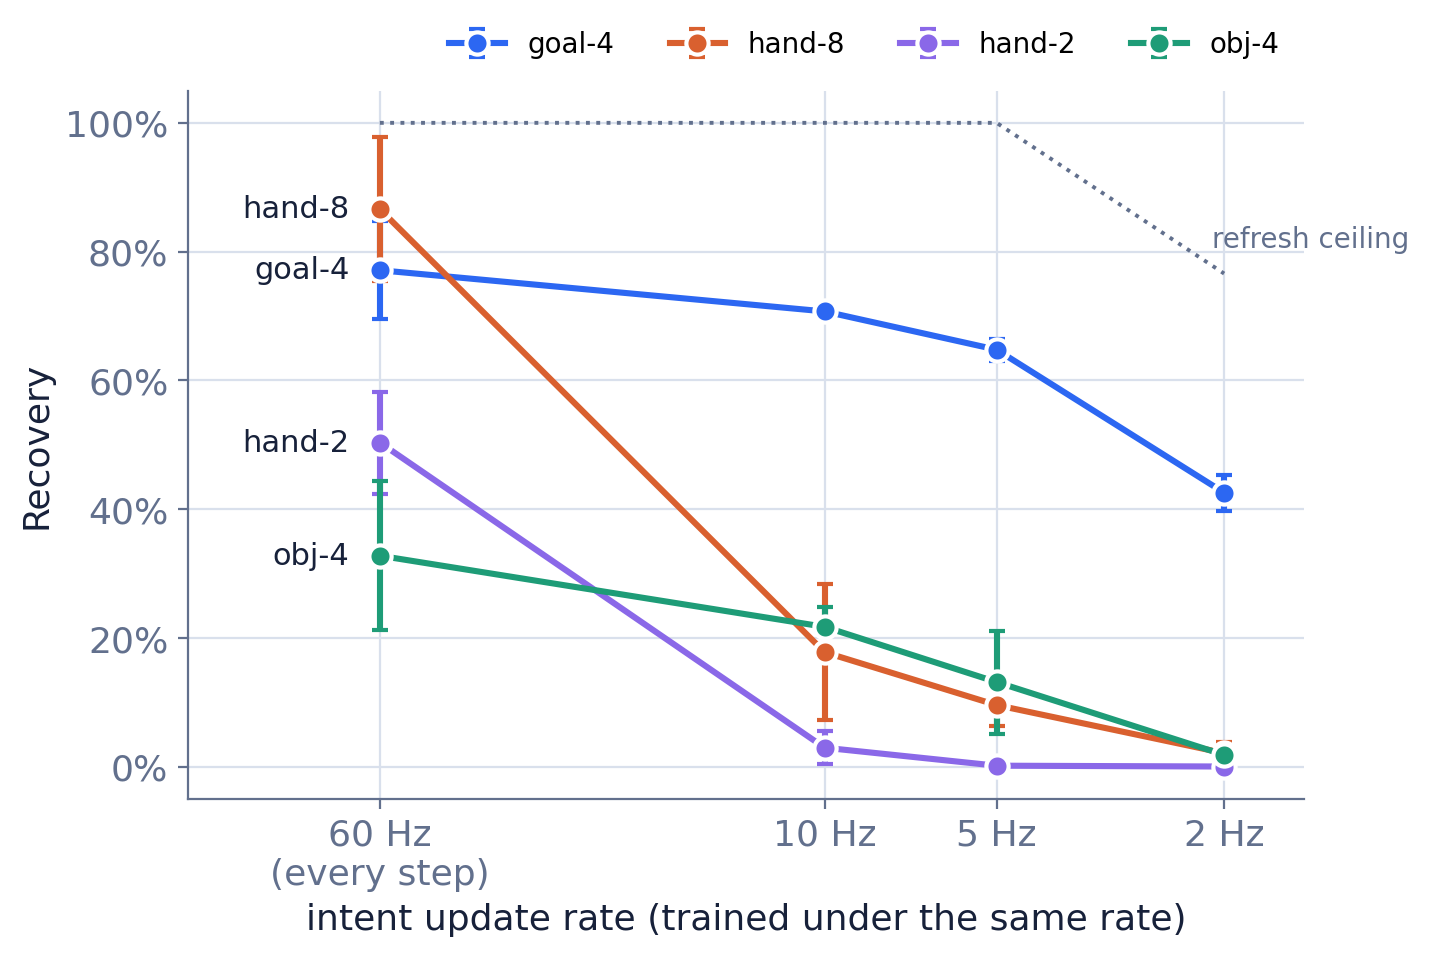
\includegraphics[width=\linewidth]{figures/rate_sweep.png}
    \caption{Rate sweep (trained under hold)}
  \end{subfigure}\hfill
  \begin{subfigure}[b]{0.60\linewidth}
    \centering
    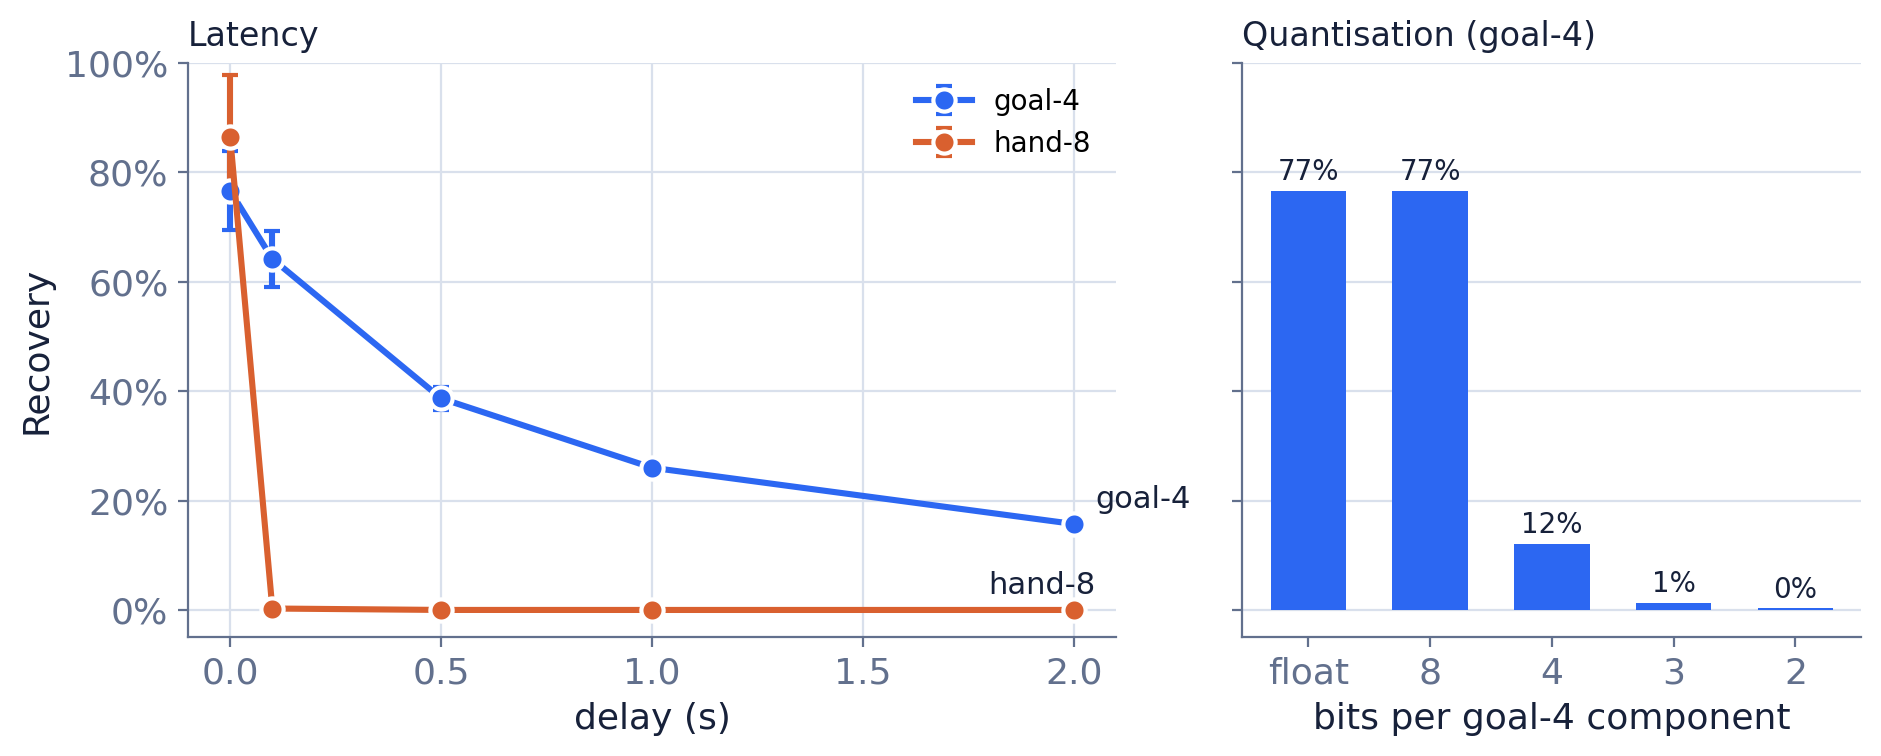
\includegraphics[width=\linewidth]{figures/channel_delay_bits.png}
    \caption{Eval-only latency and scalar quantization}
  \end{subfigure}
  \caption{Channel degradation on Task~1. (a)~Rate reversal between \texttt{goal-4} and \texttt{hand-8} across 60--2~Hz. (b)~Under latency, \texttt{hand-8} fails at 0.1~s while \texttt{goal-4} tracks Eq.~\ref{eq:waiting}; quantization requires $\ge 8$~bits/component (staleness collapse in Appendix~\ref{app:stats}).}
  \label{fig:channel_degradation}
\end{figure}

\subsection{Cross-Task Generalization and the ``Stale Goal'' Trap (Task~2: $z$-Axis)}
\label{sec:exp_m2}
On Task~2 ($P_E = 31.14$), the goal-hidden \texttt{blind} policy already reaches $P_{\mathrm{blind}} = 19.66$ (63\% of $P_E$) by exploiting a goal-free unidirectional spinning heuristic (Appendix~\ref{app:stats}).
Even so, the rate reversal replicates cleanly: at 60~Hz, \texttt{hand-8} (36.7), \texttt{hand-4} (40.1), \texttt{goal-yaw} (35.7), and \texttt{goal-4} (32.7) perform comparably ($p \ge 0.23$).
At 10~Hz, our pre-registered $n=5$ seed test confirms that task-native \texttt{goal-yaw} ($31.05 \pm 2.38$, \textbf{99.2\%} recovery) significantly outperforms \texttt{hand-8} ($23.06 \pm 4.50$, \textbf{29.6\%} recovery; Welch $p=0.0124$, Mann--Whitney $U=0, p=0.0079$).
Crucially, at 2~Hz both \texttt{goal-yaw} (16.2) and \texttt{hand-8} (11.7) fall \emph{below} \texttt{blind} (19.7; $p=0.03$ for \texttt{hand-8}), exposing a \textbf{stale-goal trap} where chasing outdated goals underperforms a goal-free heuristic.

\subsection{Multi-Skill Hinged Cube and Boundary Conditions (Task~3)}
\label{sec:exp_task3}
Table~\ref{tab:unified_v4} compares multi-skill controllers on the hinged cube.
Raw two-expert switching suffers 14--26\% handoff drops and 14--19\% turn stalls; fine-tuning the turn expert on Stage~1 \texttt{up} end states cuts drops to 1--2\% and lifts \texttt{up,turn} to 7.51 cycles/600 steps.
Resolving the v1--v3 exploits (Appendix~\ref{app:unified_debug}), \textbf{\texttt{Unified v4}} reaches \textbf{18.02} \texttt{up,turn} cycles (2 seeds: 18.88 / 17.16; $2.4\times$ tuned handoff) and 10.08 \texttt{any,up,turn} cycles with $<0.02\%$ stalls and balanced $\pm 90^\circ$ turns.

\begin{table}[t]
  \centering
  \caption{Task~3 multi-skill composition (per 600 steps, 1,024 envs). \texttt{Unified v4} (2-seed mean: 18.88 / 17.16) outperforms handoff-tuned switching by $2.4\times$ with near-zero stalls.}
  \label{tab:unified_v4}
  \footnotesize
  \setlength{\tabcolsep}{4pt}
  \begin{tabular*}{\linewidth}{@{\extracolsep{\fill}}lccccc}
    \toprule
    Controller & \texttt{up,turn} & \texttt{any,up,turn} & Stalls ($>120$) & Falls (\texttt{up,turn}) & Turn Steps (med.) \\
    \midrule
    Two-Expert (raw) & 4.61 & 3.50 & 14--19\% & 0.70 & 33--35 \\
    Two-Expert (tuned) & 7.51 & 5.48 & 3.5--4.5\% & 0.10 & 33 \\
    \textbf{\texttt{Unified v4} (2-seed mean)} & \textbf{18.02} & \textbf{10.08} & \textbf{0.02\%} & \textbf{0.013} & \textbf{18--19} \\
    \bottomrule
  \end{tabular*}
\end{table}

Multi-skill switching reproduces both Part~I laws: two-expert selector hold/delay (E2') tracks $600/(T_0+L\cdot w)$ without added drops (Appendix~\ref{app:stats}), and goal-hidden students on \texttt{Unified v4} (E3, $n=3$) reproduce the 10~Hz reversal on \texttt{up,turn} (60~Hz: \texttt{hand-8} 9.68 vs.\ \texttt{goal-7} 6.20; 10~Hz: \texttt{goal-7} retains \textbf{69\%} [4.30] vs.\ \texttt{hand-8} \textbf{4\%} [0.36], $p=0.063$; mixed-phase \texttt{any}/\texttt{goal-11} diagnostics in Appendix~\ref{app:stats}).
By contrast, an 8-seed study on isolated 1-DOF face turns (E1) reveals a \textbf{boundary condition}: take-off ($>10$ turns) is bimodal and seed-driven (4/16 for both \texttt{goal-yaw} and \texttt{hand-8}, Fisher $p=1.0$), and taken-off \texttt{hand-8} runs reach expert level even at 10~Hz (23.2--34.0 turns) despite negative action-reconstruction variance ($-7\%$).
An offline MLP probe resolves this paradox: on 1-DOF face turns, held \texttt{hand-8} at 10~Hz still retains \textbf{53\%} of hidden goal-error variance ($R^2=0.53$, vs.\ only \textbf{22\%} on 3D Task~1), effectively degenerating into a goal code (before still collapsing at 2~Hz to 13\% vs.\ 60--82\% for \texttt{goal-yaw}).

\subsection{End-to-End Visual VLM Control over Frozen \texttt{Unified v4} (Scheme~C)}
\label{sec:exp_vlm}
\paragraph{Execution ceiling and zero-shot bottlenecks.}
Wrapping frozen \texttt{Unified v4} in our 96-state external-goal interface (P2.1) yields \textbf{100.0\%} closed- and open-loop BFS execution (2,048/2,048 episodes, 0.0\% drops, 0.0\% hinge drift $>45^\circ$, 16.5 steps/macro-action) and \textbf{0.0\%} drops over 4.0~s (240-step) holds—a zero-loss physical floor ($P_{\mathrm{Oracle}}=1.000$).
On this floor, zero-shot \texttt{Qwen3-VL-8B-Instruct} (pipeline verified on EmbSpatial 78.24\% vs.\ 78.5\% official, Appendix~\ref{app:scheme_c}) exhibits two bottlenecks:
(1)~\emph{Spatial grounding}: on 180 held-out test frames (CircularEval), 3-view \texttt{montage} reaches 90.0\% on coarse \texttt{up} color but only \textbf{7.5\%} on narrow-band \texttt{band} (0.0\% all-levels), whereas adding Set-of-Mark \texttt{[1]/[2]} jumps \texttt{turned} to 80.0\% and \texttt{band} to 67.9\% (50.9\% all-levels);
(2)~\emph{Relational planning}: given oracle \texttt{relational} text state, zero-shot greedy success falls across $L=1..4$ (100\% / 56\% / 14\% / 4\%, overall 43.5\%), while Pass@8 stays at 74\%/66\%/54\%.

\paragraph{Perception generalization, overfitting audit, and forgetting check.}
Full held-out perception, benchmark, and closed-loop generalization tables appear in Appendix~\ref{app:scheme_c} (Tables~\ref{tab:vlm_perception}--\ref{tab:app_cl_gen}).
Frozen-ViT Map-then-Reason LoRA SFT (\texttt{C1-v1}, 0.51\% trainable parameters, zero SoM tags) lifts canonical \texttt{band} accuracy from 7.5\% to \textbf{99.4\%} (99.4\% \texttt{@nohand}) and generalizes strongly to swapped colors (OOD G$\leftrightarrow$B \textbf{96.2\%}), novel palettes (89.9\% \texttt{band}), and two unseen cameras (\texttt{s130+top} \textbf{83.3\%}), while preserving EmbSpatial ($-1.89\%$), MMStar ($-1.13\%$), and BLINK ($-3.84\%$).
Auditing \texttt{C1-v1} exposes format/abstention overfitting on unseen inverse prompts (\texttt{v3}: 36.8\%) and unanswerable frames (CBD: 0.0\%); our data-centric \textbf{\texttt{C1-v2}} (1 epoch, multi-template + CBD + 30\% augmentation + cyclic $\mathbb{Z}_4$ CoT) maintains 98.7\% canonical and 96.2\% OOD accuracy while lifting CBD abstention to \textbf{100.0\% (21/21)} (0.6\% false-CBD), unseen \texttt{v3} to \textbf{59.2\%} (\texttt{turned} 96.7\%), and open-loop \texttt{turn} optimality from 77.1\% to \textbf{89.6\%}.

\paragraph{Closed-loop manipulation, GRPO saturation, and real 60~Hz Isaac Lab verification.}
Table~\ref{tab:vlm_closedloop} summarizes multi-turn closed-loop control across all 96 states.
On the 200-task image pool, \texttt{C1-v1} reaches \textbf{100.0\% (181/181)} at 1.216$\times$ rounds with zero illegal actions because closed-loop visual feedback self-corrects occasional $\pm 90^\circ$ sign flips; consequently, outcome-reward GRPO (\texttt{C2}) hits DAPO zero-variance saturation (74--82\% all-pass groups), whereas explicit cyclic CoT in \texttt{C1-v2} cuts the rounds ratio to \textbf{1.121$\times$}.
Deploying \texttt{C1-v1} in \textbf{real 60~Hz Isaac Lab online 3-camera rendering} over 128 physical episodes ($L=1..4$, 32/level, 368 rounds) achieves \textbf{100.0\% (128/128)} success, \textbf{0.0\% falls}, \textbf{98.9\%} live 96-state accuracy, \textbf{1.175$\times$} rounds ratio, and \textbf{15.7 steps (0.26~s)} per macro-action—matching the BFS Oracle with zero sim-to-offline gap.

\begin{table}[t]
  \centering
  \caption{Multi-turn closed-loop manipulation over frozen \texttt{Unified v4} (offline 200-task image pool and real 60~Hz Isaac Lab online 3-camera physics).}
  \label{tab:vlm_closedloop}
  \footnotesize
  \setlength{\tabcolsep}{3.5pt}
  \begin{tabular*}{\linewidth}{@{\extracolsep{\fill}}lcccccc}
    \toprule
    Method / Eval Env & Eps & Success & Falls & Rounds/$L^*$ & State Acc & Illegal \\
    \midrule
    Zero-Shot Text (Oracle) & 200 & 43.5\% & --- & --- & (Oracle text) & --- \\
    BFS Oracle (Isaac Lab \texttt{v4}) & 2,048 & \textbf{100.0\%} & 0.0\% & 1.000$\times$ & (Oracle sim) & 0.0\% \\
    \midrule
    \texttt{C1-v1} (200-Task Pool) & 181 & \textbf{100.0\%} & --- & 1.216$\times$ & 91.7\% & 0.0\% \\
    \texttt{C2} GRPO (Gnd./Term., Pool) & 182 / 181 & \textbf{100.0\%} & --- & 1.236 / 1.216$\times$ & 90.2 / 91.5\% & 0.0\% \\
    \texttt{C1-v2} (200-Task Pool) & 181 & 98.9\% & --- & \textbf{1.121$\times$} & 90.5\% & 0.4\% \\
    \textbf{\texttt{C1-v1} (Isaac Lab Online)} & \textbf{128} & \textbf{100.0\%} & \textbf{0.0\%} & \textbf{1.175$\times$} & \textbf{98.9\%} & \textbf{0.0\%} \\
    \bottomrule
  \end{tabular*}
\end{table}

\section{Discussion, Limitations, and Conclusion}
\label{sec:conclusion}

\subsection{Key Takeaways for Slow-Planner to Fast-Hand Design}
Our experiments across three Shadow Hand tasks yield three clear takeaways for pairing slow planners with fast dexterous hands:
\begin{itemize}[leftmargin=1.5em,itemsep=1pt,topsep=1pt]
  \item \textbf{Keep the hand fast; send goals, not actions or waypoints.} A 20-DOF hand cannot run directly at 2--10~Hz (Slow Expert $\le 15\%$ at 10~Hz, $0\%$ at 2~Hz), and held action synergies or moving waypoints go stale within steps. The low-level controller must close its proprioceptive loop at 60~Hz while the slow planner sends goal-level targets---except on simple 1-DOF tasks where action codes implicitly encode the goal direction.
  \item \textbf{Match precision and latency to task dynamics.} Two task properties set the channel budget: success tolerance sets precision ($\ge 8$~bits/component for 0.1~rad), and zero-wait goal time $T_0$ sets latency ($d \ll T_0$ under $P(d)\approx 600/(T_0+d)$). Moreover, when a task admits a goal-free heuristic (Task~2), sending an outdated goal is strictly worse than sending no goal at all.
  \item \textbf{Lightweight spatial grounding suffices once a 60~Hz skill layer exists.} Given a reliable goal-conditioned controller (\texttt{Unified v4}), an open-weight 8B VLM is bottlenecked by fine-grained spatial grounding rather than vision features. Frozen-ViT Map-then-Reason LoRA resolves grounding with minimal forgetting, while multi-template phrasing and abstention data prevent format overfitting.
\end{itemize}

\subsection{Limitations and Future Work}
Three limitations highlight clear next steps:
(1)~\textbf{Single-camera partial observability:} closed-loop visual evaluation uses three fixed cameras (\texttt{c1+s040+s220}); extending to one occluded camera requiring exploratory \texttt{reorient} moves is a natural POMDP extension.
(2)~\textbf{Asynchronous timing and sim-to-real:} physics pauses during VLM decoding; real-time asynchronous inference (testing Eq.~\ref{eq:waiting}), physical perturbations, and hardware transfer remain future work.
(3)~\textbf{Over-abstention on top-bar cues and seed breadth:} on unseen \texttt{v3} queries, \texttt{C1-v2} still over-abstains (26.3\%) when relying on the top face's black orientation bar rather than side strips; additionally, \texttt{Unified v4} uses 2 seeds and auxiliary interface grids use 3 seeds (core rate-reversal claims use $n=5$).

\subsection{Conclusion}
Returning to our central question, a slow planner should transmit \emph{goal-level} targets---not action synergies or moving waypoints---to a fast 60~Hz dexterous hand.
Channel degradation separates viable from brittle interfaces decisively: while 8-D action synergies match goals at 60~Hz, low refresh rates ($\le 10$~Hz) and latency ($\ge 0.1$~s) collapse action and waypoint codes via inter-update staleness, leaving goal commands---at $\ge 8$~bits/component to meet the 0.1~rad tolerance---as the only representation that degrades predictably along the waiting-time law.
Guided by this principle, pairing a frozen 60~Hz goal-conditioned controller (\texttt{Unified v4}) with lightweight Map-then-Reason LoRA on \texttt{Qwen3-VL-8B-Instruct} achieves 100.0\% (128/128) zero-drop closed-loop manipulation in Isaac Lab, showing that the right goal-level interface turns a slow, open-weight VLM into a reliable dexterous-hand planner.


% References do not count toward the 5--8 page limit
\clearpage
\bibliographystyle{plainnat}
\bibliography{references}

% Appendices do not count toward the 5--8 page limit
\clearpage
\appendix
\section{Declaration of Generative AI Use}
\label{app:ai_declaration}
During the preparation of this project and report, the authors used generative AI tools---specifically GPT~6, Fable~5.2, Opus~5.5, and Gemini~4 (Carbon, Argon, Neon, and Hydrogen)---for discovering and summarizing relevant literature, English language polishing, LaTeX formatting, and assisting with drafting, refactoring, and debugging auxiliary engineering, Slurm, data-processing, and visualization scripts. All core research ideas, experimental designs, analyses, and scientific conclusions are the authors' own work. Every AI-assisted code snippet, text revision, and literature reference was critically reviewed, tested, and verified by the authors against primary sources, and all reported results and figures originate strictly from real experiments conducted by the team on the NUS SoC compute cluster. The authors take full responsibility for the content, accuracy, and academic integrity of this submission.

\section{Implementation Details and Code Reproducibility}
\label{app:impl}
All code, Slurm scripts, environment definitions, and result summaries are publicly available at \url{https://github.com/ziyouledi/CS5478_project} (see repository \texttt{README.md} and \texttt{Experiment Plan/cluster\_smoke/README.md} for end-to-end reproduction instructions).

\paragraph{Runtime and hardware.}
Simulation and RL runs use Isaac Lab v2.3.1 (commit \texttt{5c2ec81c}), Isaac Sim 5.1.0.0, Python 3.11.17, PyTorch 2.7.0+cu128, and RL-Games 1.6.1 on NUS SoC Slurm GPU nodes (NVIDIA Tesla T4 15~GB for 2,048-env training/evaluation; NVIDIA H200 141~GB for 8,192-env \texttt{Unified v4} training).
VLM inference and LoRA training run on NVIDIA H100 (47/96~GB) using vLLM 0.11.0, PyTorch 2.8.0, and Transformers 4.57.6.

\paragraph{PPO and asymmetric critic hyperparameters.}
All Stage 1, M1, M2, and rate-sweep PPO runs train for 5,000 iterations with 2,048 parallel environments (163.84M transitions, horizon 16, minibatch 32,768, 5 mini-epochs, adaptive learning rate $5\times 10^{-4}$, target KL 0.016, actor MLP \texttt{[512, 512, 256, 128]} with ELU).
In goal-hidden stages (M1, M2-hidden, E1, E3), the 8 goal observation entries \texttt{obs[64:72]} (\texttt{goal\_rot} and \texttt{quat\_mul(object\_rot, conj(goal\_rot))}) are removed from the actor while \texttt{central\_value\_config} receives the full clipped 157-D state with matching network architecture, minibatch size, and 5 mini-epochs.
Frozen experts are verified by SHA-256 checksums before every rollout and student run; all learning curves evaluate 25 checkpoints (every 200 iterations) over 1,024 deterministic episodes.

\section{Stage 1 (Goal-Visible) Results and Spectral Diagnostics}
\label{app:stage1}
Table~\ref{tab:app_stage1} summarizes Stage 1 goal-visible learning efficiency on Task 1 (21 runs, $P_E=26.11$) and Task 2 M2 (30 runs including \texttt{joint-2/4}, $P_E=31.14$).
When the actor observes the goal directly, no intent condition differs significantly from \texttt{blind} (Task 1 one-way ANOVA N80 $p=0.82$, AUC $p=0.65$; Task 2 ANOVA N80 $p=0.90$, AUC $p=0.82$, final $p=0.69$; with a 4th seed on \texttt{blind}/\texttt{hand-2}/\texttt{joint-2}, \texttt{hand-2} vs.\ \texttt{blind} AUC Welch $p=0.060$ remains non-significant).
On Task 2, \texttt{joint-$k$} (projecting expert actions onto the joint-position PCA basis) captures less action variance than action PCA (38.1\% vs.\ 42.7\% at $k=2$; 55.9\% vs.\ 64.0\% at $k=4$) and does not outperform \texttt{hand-$k$}.
Diagnostic PCA on measured 24-D joint positions on Task~1 confirms that high dimensionality is intrinsic rather than a bang-bang artifact: joint positions are much smoother (6.2\% at limits vs.\ 62.2\% for actions; 5.2\% sign flips vs.\ 20.4\%), yet still require 15 components for 95\% variance (11 on Task~2), decorrelate within 2.4--6 control steps, and require 92--100 components to explain 95\% of a 21-step goal segment.

\begin{table}[h]
  \centering
  \caption{Stage 1 (goal-visible) learning efficiency: N80 (iterations to $0.8 P_E$), normalized AUC, and final normalized score ($n=3$ seeds per condition). No condition is statistically distinguishable from \texttt{blind}.}
  \label{tab:app_stage1}
  \small
  \begin{tabular}{lcccccc}
    \toprule
    & \multicolumn{3}{c}{Task 1: $\mathrm{SO}(3)$ ($P_E=26.11$)} & \multicolumn{3}{c}{Task 2: $z$-Axis M2 ($P_E=31.14$)} \\
    \cmidrule(lr){2-4}\cmidrule(lr){5-7}
    Condition & N80 (iter) & AUC & Final/$P_E$ & N80 (iter) & AUC & Final/$P_E$ \\
    \midrule
    \texttt{blind} & 2375 & 0.695 & 0.974 & 1699 & 0.824 & 1.097 \\
    \texttt{wrist-2} & 2278 & 0.708 & 0.962 & 1168 & 0.966 & 1.201 \\
    \texttt{hand-2} & 1994 & 0.786 & 0.986 & 1087 & 1.062 & 1.409 \\
    \texttt{hand-4} & 2361 & 0.696 & 0.945 & 2126 & 0.761 & 1.111 \\
    \texttt{hand-20} & 2147 & 0.745 & 0.946 & 2113* & 0.922 & 1.124 \\
    \texttt{obj-1} & 1842 & 0.765 & 1.018 & 1566 & 0.906 & 1.293 \\
    \texttt{obj-4} & 2664 & 0.684 & 0.932 & 1556 & 0.861 & 1.126 \\
    \texttt{joint-2} & --- & --- & --- & 1072 & 0.958 & 1.269 \\
    \texttt{joint-4} & --- & --- & --- & 1572 & 0.920 & 1.227 \\
    \bottomrule
  \end{tabular}
\end{table}

\begin{table}[h]
  \centering
  \caption{Equal-budget PCA variance retention and wrist--finger coupling analysis on 20-D expert actions ($1{,}228{,}800$ transitions; Jobs~\texttt{1024096}, \texttt{1033179}, \texttt{1153641}). Spending 2 uncompressed dimensions on the wrist (only 15.5\% of Task~1 and 11.9\% of Task~2 variance) consistently retains less total action variance---and yields lower 60~Hz M1 recovery---than joint whole-hand PCA (\texttt{hand-$k$}) at every budget $k \in \{2,4,8\}$. In Task~1, wrist loading peaks on PC3 (59.0\% of squared loading) with wrist--finger canonical correlations $0.72, 0.50$ (mean $|r|=0.11/0.15$ vs.\ finger--finger $0.14$; Task~2: $0.84, 0.71$, mean $|r|=0.20/0.22$ vs.\ $0.18$).}
  \label{tab:app_pca}
  \small
  \resizebox{\linewidth}{!}{%
  \begin{tabular}{ccccccc}
    \toprule
    & \multicolumn{2}{c}{Task~1 ($\mathrm{SO}(3)$) Variance Retained} & \multicolumn{2}{c}{Task~1 M1 60~Hz Recovery} & \multicolumn{2}{c}{Task~2 ($z$-Axis) Variance Retained} \\
    \cmidrule(lr){2-3}\cmidrule(lr){4-5}\cmidrule(lr){6-7}
    Dim $k$ & \texttt{hand-$k$} (Total / Wrist) & \texttt{wrist2-finger-$(k{-}2)$} & \texttt{hand-$k$} & \texttt{wrist2-finger-$(k{-}2)$} & \texttt{hand-$k$} (Total / Wrist) & \texttt{wrist2-finger-$(k{-}2)$} \\
    \midrule
    2 & \textbf{35.8\%} / 14.2\% & 15.5\% (\texttt{wrist-2}) & \textbf{0.504} & 0.292 & \textbf{42.7\%} / 57.7\% & 11.9\% (\texttt{wrist-2}) \\
    4 & \textbf{56.8\%} / 63.6\% & 49.9\% (\texttt{wrist2-finger-2}) & \textbf{0.714} & 0.550 & \textbf{64.0\%} / 70.3\% & 49.2\% (\texttt{wrist2-finger-2}) \\
    8 & \textbf{81.1\%} / 93.1\% & 78.1\% (\texttt{wrist2-finger-6}) & \textbf{0.866} & 0.653 & \textbf{83.9\%} / 80.7\% & 79.5\% (\texttt{wrist2-finger-6}) \\
    \bottomrule
  \end{tabular}%
  }
\end{table}

\section{Unified Multi-Skill Policy Debugging Progression (v1 $\to$ v4)}
\label{app:unified_debug}
Achieving reliable single-policy multi-skill control on the hinged cube required systematically diagnosing and eliminating three RL exploits:
\begin{itemize}[leftmargin=1.5em,itemsep=2pt]
  \item \textbf{v1 (static detent reward exploit):} Including an inverse-distance hinge term $1/(|\Delta\phi|+0.1)$ during all phases paid $+10$/step simply for holding the cube still ($\approx 6,000$/episode), causing the policy to freeze (3 goals across 1,024 envs).
  \item \textbf{v2 (directional stall and boundary parking):} Restricting the inverse-distance term to the active phase enabled strong reorientation (\texttt{any} 21.2, \texttt{up} 27.5), but 75--85\% of \texttt{turn} phases stalled ($>120$ steps) even after 10,000 iterations. Per-step trace diagnostics and a zero-detent torque probe revealed two split failures: $+90^\circ$ turns were never attempted (median excursion $0.7^\circ$ even at 0~N$\cdot$m detent), while $-90^\circ$ turns reached the hinge target in 10 steps and then parked outside the 0.4~rad cube-orientation tolerance to harvest $+9.1$/step indefinitely without closing the phase.
  \item \textbf{v3 (phase-scheduler tilt exploit):} Replacing static distance with progress shaping eliminated parking, yet turn stalls rose to 99.5\% (\texttt{up,turn} 0.50 cycles). Trace analysis proved a Markov scheduler exploit: when \texttt{is\_turn} activated, the policy tilted the cube past 0.4~rad within 5 steps so that at the 120-step timeout the scheduler drew a lucrative reorientation phase instead of another turn, matching the exact analytical steady-state return ($\approx 2,863$ vs.\ observed $2,818$).
  \item \textbf{v4 (solved):} Terminating the episode on 120-step phase timeout ($V(s')=0$), initializing 50\% of resets into $\pm 90^\circ$ turn phases from Stage 1 \texttt{up} handoff states, and adding monotonic hold-milestone shaping ($+5$ per new max hold step, cap $+50$) with fall penalty $-15$ eliminated all exploits, lifting \texttt{up,turn} to 18.88 (seed 0) and 17.16 (seed 1) cycles/600 steps with $<0.02\%$ stalls.
\end{itemize}

\section{Extended Statistical Tests, Controls, and E3 Diagnostics}
\label{app:stats}
\paragraph{Task 1 ($n=5$ seeds) and Task 2 ($n=5$ seeds) controls and rate-reversal tests.}
At 60~Hz on Task~1, wrist--finger decoupling (\texttt{wrist2-finger-2}: $0.550\pm 0.080$, AUC $0.356$; \texttt{wrist2-finger-6}: $0.653\pm 0.172$; Table~\ref{tab:app_pca}) does not outperform joint whole-hand PCA (\texttt{hand-8}: $0.866\pm 0.112$, $p=0.16$; at 10~Hz: $0.269$ vs.\ $0.178$, $p=0.38$).
On Task 1, \texttt{goal-4} vs.\ \texttt{hand-8} Recovery is $0.78$ vs.\ $0.80$ at 60~Hz (Welch $p=0.86$), $0.71$ vs.\ $0.19$ at 10~Hz ($p=0.0003$), and $0.44$ vs.\ $0.025$ at 2~Hz ($p<0.0001$).
Resuming all five 10~Hz \texttt{hand-8} runs from 5,000 to 10,000 iterations lifts recovery only from $0.19$ to $0.22$ (flat after 8,000 iterations, $U=0$ vs.\ 60~Hz), ruling out under-training; under eval-only 10~Hz hold, 60~Hz \texttt{hand-8} drops from $0.87$ to $0.03$ with 62\% cube drops.
Training \texttt{goal-4} under large delays ($d=30/60$) underperforms evaluating a zero-delay policy under the same delay ($0.26/0.19$ vs.\ $0.39/0.26$, $p\le 0.0013$); zero-delay cross-checks confirm delay-trained students learn a slower controller ($T_0 \approx 60$ vs.\ 30 steps).
Resuming \texttt{goal-4} to 10,000 iterations passed our pre-registered transient check (mean iterations 5,200--5,600 $= 1.024\times$ own iteration-5,000 score).
On Task 2, \texttt{blind} spins unidirectionally (angular-velocity sign consistency $\ge 0.99$, 9--11 turns/episode, vs.\ $<0.1$ for goal-informed policies); eval-only delay drops \texttt{goal-yaw} below \texttt{blind} beyond $\approx 0.23$~s.
At 10~Hz (pre-registered Block 3b, $n=5$), \texttt{goal-yaw} ($31.05\pm 2.38$, Recovery 0.992) beats \texttt{hand-8} ($23.06\pm 4.50$, Recovery 0.296) with Welch $p=0.0124$ and Mann--Whitney $U=0$ ($p=0.0079$); \texttt{goal-4} ($27.96\pm 1.81$, Recovery 0.724) vs.\ \texttt{hand-8} gives $p=0.0704$.
On Task~3 E2', sweeping selector hold ($N=6,30$) and delay ($d=6,30,60$) on tuned two-expert switching closely follows $600/(T_0+L\cdot w)$ (within 3--7\% on \texttt{up,turn} at $d=30,60$) without increasing drops.

\begin{figure}[h]
  \centering
  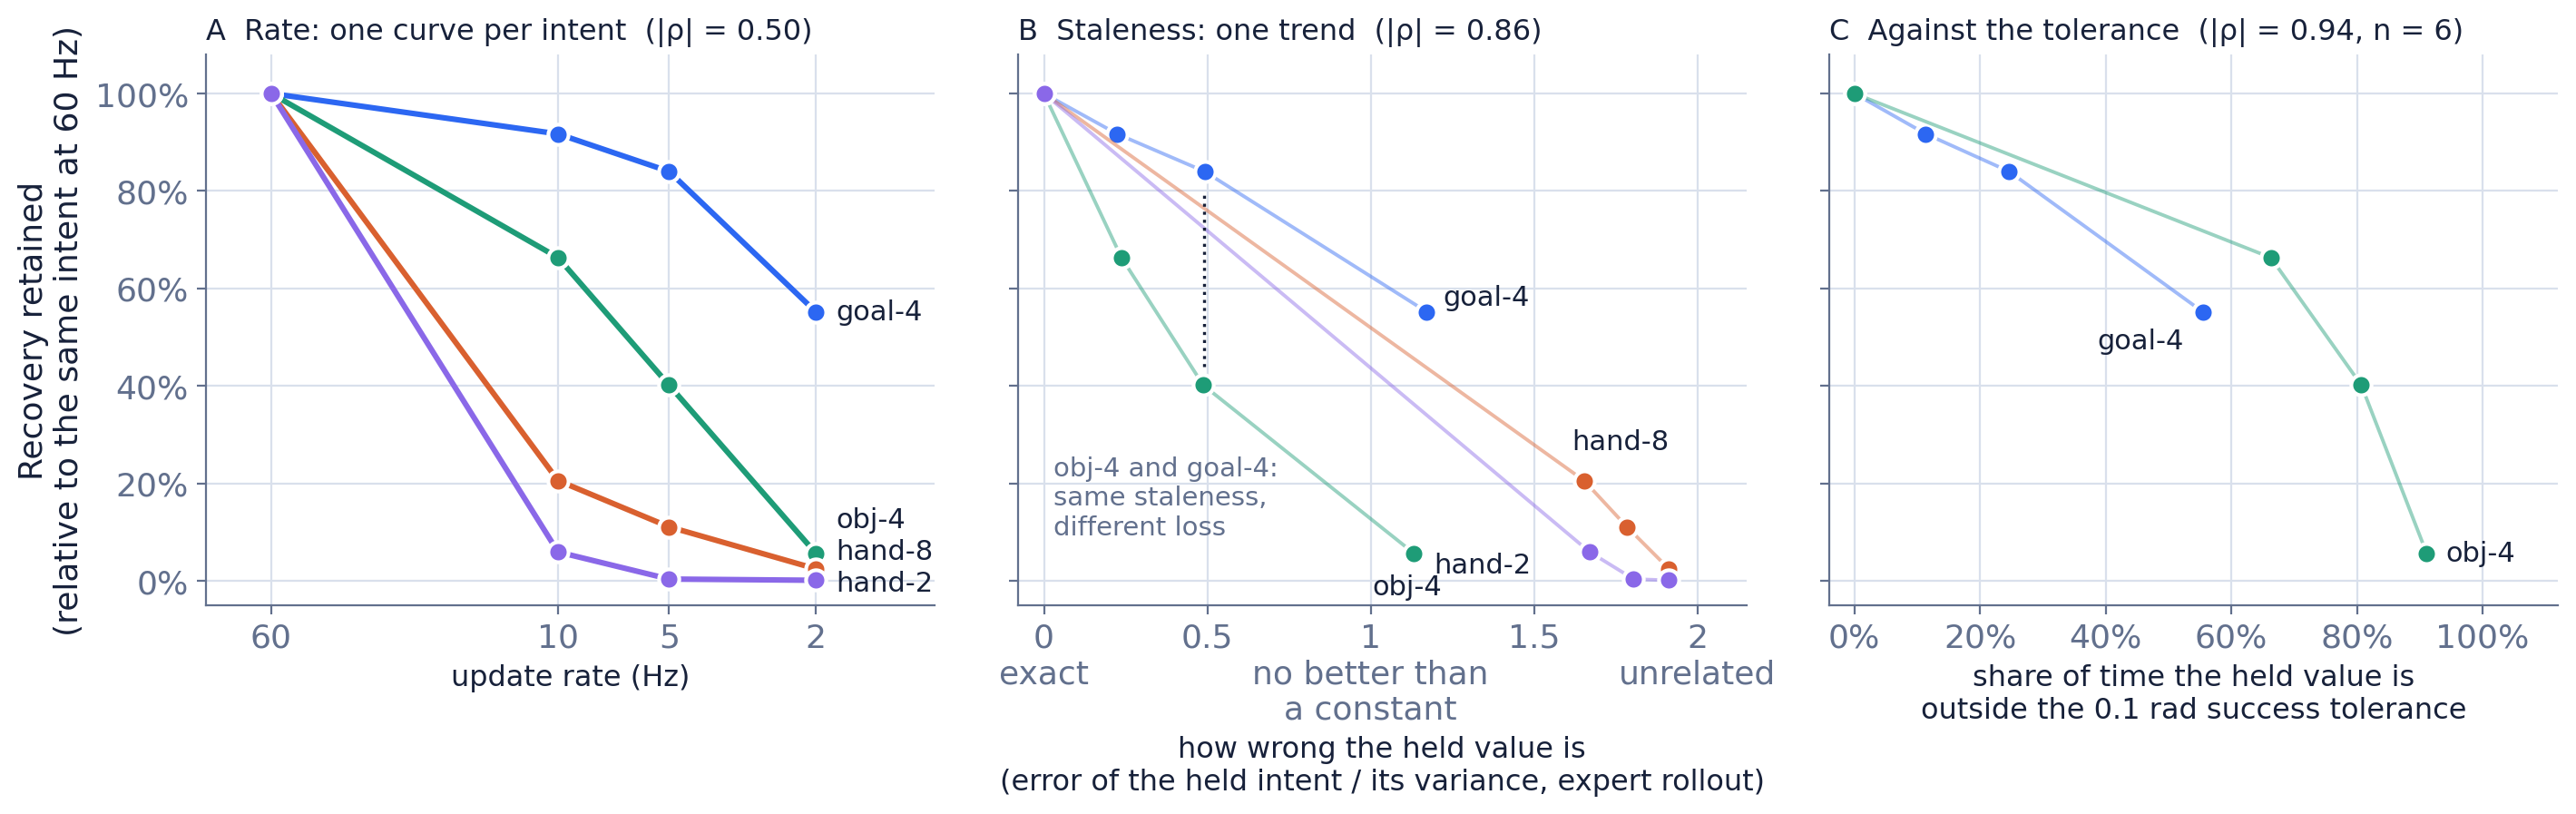
\includegraphics[width=\linewidth]{figures/staleness.png}
  \caption{Unified inter-update staleness collapse on Task~1. Plotting retained recovery against update rate (A) yields separate curves per interface ($|\rho|=0.50$), whereas plotting against normalized inter-update staleness (B, $|\rho|=0.86$) and fraction of steps outside the 0.1~rad success tolerance (C, $|\rho|=0.94$) collapses all interfaces onto a single monotonic trend.}
  \label{fig:app_staleness}
\end{figure}

\paragraph{E3 \texttt{any}-goal diagnostics.}
On \texttt{Unified v4}, masking \texttt{obs[68:72]} (relative rotation) drops the frozen teacher's \texttt{any}/\texttt{up} throughput from 29.4/50.0 to 0.03, whereas masking the goal quaternion alone keeps 25.3/45.8.
Removing the 120-step timeout (V1) still fails to learn \texttt{any} (0.003--0.028), while training \texttt{any}-only with timeout (V2) succeeds (3.0--4.6), implicating mixed-goal interference.
Appending \texttt{obs[68:72]} (\texttt{goal-11}, 6 seeds) yields 2/6 seeds learning \texttt{any} (vs.\ 0/6 for \texttt{goal-7}, Fisher one-sided $p=0.23$) and significantly higher \texttt{up} completions (15.1--31.1 vs.\ 8.1--14.8, MWU $p=0.002$, Welch $p=0.029$).

\section{Complete Scheme C Perception, Benchmark, and Open-Loop Audit Tables}
\label{app:scheme_c}

\begin{table}[h]
  \centering
  \caption{Held-out Z1 180-frame perception and overfitting-boundary audit (\texttt{test} split, 3-view \texttt{montage}, zero SoM tags, CircularEval). \texttt{C1-v1} generalizes visually; \texttt{C1-v2} repairs abstention (CBD) and unseen prompt \texttt{v3}.}
  \label{tab:vlm_perception}
  \small
  \setlength{\tabcolsep}{4.5pt}
  \resizebox{\linewidth}{!}{%
  \begin{tabular}{lcccccc}
    \toprule
    Model & Canonical All/\texttt{band} & \texttt{@nohand} & OOD G$\leftrightarrow$B & Novel Palette \texttt{band} & Unseen \texttt{v3} All/\texttt{turned} & Unans.\ CBD ($n=21$) \\
    \midrule
    Zero-shot \texttt{Qwen3-VL-8B} & --- / 7.5\% & --- / 5.7\% & --- & --- & --- & 52.4\% \\
    \texttt{C1-v1} (2 ep, Map-then-Reason) & \textbf{99.4} / \textbf{99.4\%} & \textbf{99.4\%} & \textbf{96.2\%} & 89.9\% & 36.8 / 60.0\% & 0.0\% \\
    \textbf{\texttt{C1-v2}} (1 ep, +CBD/+tpl/+CoT) & 98.7 / 98.7\% & 96.9\% & \textbf{96.2\%} & \textbf{93.7\%} & \textbf{59.2} / \textbf{96.7\%} & \textbf{100.0\%} \\
    \bottomrule
  \end{tabular}%
  }
\end{table}

\begin{table}[h]
  \centering
  \caption{Zero-shot Z1 visual-mode ablation on \texttt{Qwen3-VL-8B-Instruct} (180 \texttt{test} frames, \texttt{c1+s040+s220}, CircularEval; vanilla in parentheses). Only Set-of-Mark (\texttt{som}) unlocks \texttt{band} zero-shot, proving spatial grounding is the bottleneck.}
  \label{tab:app_z1_modes}
  \small
  \begin{tabular}{lccccc}
    \toprule
    Question & \texttt{raw} & \texttt{crop} & \texttt{montage} & \texttt{seam} & \texttt{som} \\
    \midrule
    \texttt{up} & 0.806 (0.928) & 0.861 (0.967) & \textbf{0.900} (0.939) & 0.878 (0.967) & 0.867 (0.961) \\
    \texttt{turned} & 0.178 (0.517) & 0.100 (0.633) & 0.311 (0.689) & 0.228 (0.706) & \textbf{0.800} (0.800) \\
    \texttt{band} ($n=159$) & 0.069 (0.226) & 0.031 (0.239) & 0.075 (0.151) & 0.075 (0.195) & \textbf{0.679} (0.792) \\
    \texttt{all\_levels} & 0.000 & 0.000 & 0.000 & 0.025 & \textbf{0.509} \\
    \bottomrule
  \end{tabular}
\end{table}

\begin{table}[h]
  \centering
  \caption{Public spatial benchmark retention after frozen-ViT LoRA SFT (\texttt{C1-v1}, Job \texttt{1175804}) vs.\ base \texttt{Qwen3-VL-8B-Instruct} (Job \texttt{1166604}). Truncation drops from 6.6--7.8\% to 0.0\%.}
  \label{tab:app_public_bench}
  \small
  \resizebox{\linewidth}{!}{%
  \begin{tabular}{lrrrr}
    \toprule
    Benchmark (Questions) & Base Greedy / Qwen & \texttt{C1-v1} Greedy / Qwen & $\Delta$ (Greedy / Qwen) & Mean Tokens (Base $\to$ SFT) \\
    \midrule
    EmbSpatial (3,640) & 78.24\% / 78.38\% & \textbf{76.35\%} / \textbf{76.43\%} & $-1.89\%$ / $-1.95\%$ & $9.5 \to 9.6$ \\
    MMStar (1,500) & 67.87\% / 69.27\% & \textbf{66.73\%} / \textbf{67.33\%} & $-1.13\%$ / $-1.93\%$ & $479.9 \to 6.1$ \\
    BLINK (1,901) & 67.02\% / 66.91\% & \textbf{63.18\%} / \textbf{62.70\%} & $-3.84\%$ / $-4.21\%$ & $357.7 \to 5.1$ \\
    \bottomrule
  \end{tabular}%
  }
\end{table}

\begin{table}[h]
  \centering
  \caption{Open-loop 96-state perception ($n=180$) and BFS macro-action optimality ($n=360$, $L=1..4$) across Scheme C variants. Unseen-camera \texttt{C1-v1} perception: \texttt{c1} 96.1\%, \texttt{s040+s220} 96.8\%, \texttt{s130+top} (unseen) 83.3\%, \texttt{top} 47.1\%.}
  \label{tab:app_openloop}
  \small
  \resizebox{\linewidth}{!}{%
  \begin{tabular}{lcccccc}
    \toprule
    Model & 96-State Can./OOD & Action Opt. & \texttt{reorient} ($n=264$) & \texttt{turn} ($n=96$) & $L1/L2/L3/L4$ Opt. \\
    \midrule
    \texttt{color\_invariant} (no plan SFT) & 71.7\% / 65.0\% & 0.0\% & 0.0\% & 0.0\% & --- \\
    \texttt{C1-v1} (\texttt{vision\_full}) & 87.2\% / \textbf{90.0\%} & 93.1\% & \textbf{98.9\%} & 77.1\% & 98.0 / 79.8 / 99.0 / \textbf{100.0\%} \\
    \texttt{C2-Grounded} GRPO & 88.3\% / 88.9\% & 92.8\% & 98.5\% & 77.1\% & 97.0 / 79.8 / 99.0 / \textbf{100.0\%} \\
    \texttt{C2-Terminal} GRPO & 87.8\% / \textbf{90.0\%} & 93.1\% & \textbf{98.9\%} & 77.1\% & 98.0 / 79.8 / 99.0 / \textbf{100.0\%} \\
    \textbf{\texttt{C1-v2} (cyclic turn CoT)} & \textbf{88.9\%} / 87.2\% & \textbf{96.1\%} & 98.5\% & \textbf{89.6\%} & 97.0 / \textbf{91.7} / \textbf{100.0} / 96.2\% \\
    \bottomrule
  \end{tabular}%
  }
\end{table}

\begin{table}[h]
  \centering
  \caption{Zero-shot 60~Hz Isaac Lab closed-loop generalization suite for \texttt{C1-v2} over frozen \texttt{Unified v4} (Jobs~\texttt{1177273}, \texttt{1177367}, \texttt{1177677}, \texttt{1177987}).}
  \label{tab:app_cl_gen}
  \small
  \resizebox{\linewidth}{!}{%
  \begin{tabular}{lcccc}
    \toprule
    Zero-Shot Perturbation & Protocol & Physical Success & Live 96-State Acc. & Key Finding / Failure Mode \\
    \midrule
    10$\times$ dark low-light (\texttt{intensity=200}) & 32 eps ($L{=}1..4$) & \textbf{100.0\%} (32/32) & \textbf{100.0\%} (80/80) & 1.000$\times$ optimal rounds, 0\% drops \\
    Warm-dim (\texttt{650}) / cool-bright (\texttt{3400}) & Demo episodes & \textbf{100.0\%} & \textbf{100.0\%} & Optimal rounds, 0\% drops \\
    OOD G$\leftrightarrow$B swapped cube (USD shader) & Demo episode & \textbf{100.0\%} (3/3 rds) & \textbf{100.0\%} & Optimal rounds, 0\% drops \\
    Pure casual prompt (no Map-then-Reason) & 32 eps ($L{=}1..4$) & 18.8\% (6/32) & 0.0\% & $L{=}1$: 75\% (6/8); $L{\ge}2$: 0\% (skips map) \\
    Novel palette (\texttt{orange/cyan/purple/pink}) & Demo episode & 0.0\% & 0.0\% & Perception 93.7\%, but pink$\leftrightarrow$white \& canonical CoT \\
    \bottomrule
  \end{tabular}%
  }
\end{table}


\end{document}
